\section{Конструкция лифтов}

	\subsection{Общая схема лифта}
		Конструктивные исполнения лифтовых систем могут быть различны.
			В устройстве любого лифта обязательно присутствуют определенные компоненты,
			такие как кабина (или платформа), она закрепляется на стальных тросах,
			перекинутых через шкив приводного механизма, передающего силу с одного места на другое.
			В машинном отделении в верхней части шахты лифта расположен сам приводной механизм
			вместе с аппаратурой управления лифтом, куда и передаются сигналы из кабины лифта. 

		Внутри кабины, а также на этажах, обслуживаемых лифтом, в местах остановки лифта
			пользователь может выбрать необходимое ему направление движения - выбрать нужный
			этаж внутри кабины, либо направление вверх или вниз при вызове кабины на этаже.
			Сигнал, последовавший после нажатия какой-либо кнопки (вызова или приказа),
			передается на устройство управления лифтом. Устройством отправляется  ответное
			сообщение пользователю, подтверждающее прием команды, после чего устройство направляет
			кабину в нужном направлении, соответствующем запросу. Помимо приказного поста внутри
			кабины лифта находится кнопка аварийного вызова, с помощью которой пользователь может
			в аварийном случае установить связь с управляющим пунктом.
			Более подробно схематическое строение лифта представлено на рисунке \ref{dk1}.

			\begin{figure}[h]
				\centering
				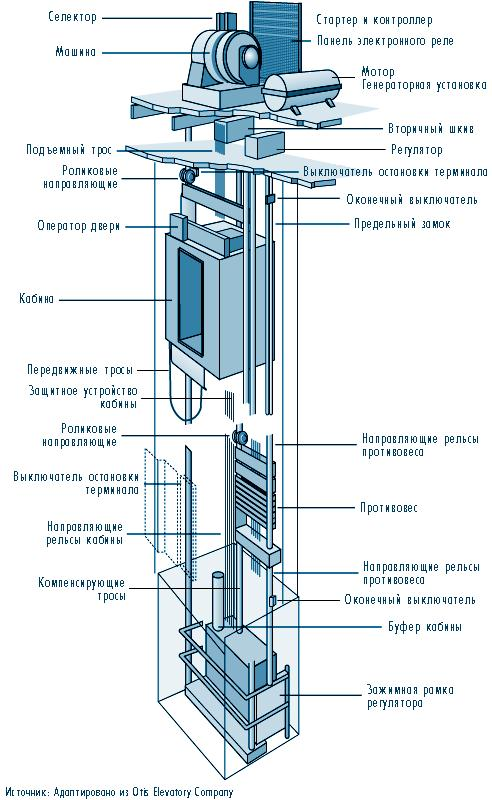
\includegraphics[width=100mm]{src/pictures/domainknowledge.png}
				\caption{Схема устройства лифтового оборудования}\label{dk1}
			\end{figure}
		% Рис. 1 - Схема устройства лифтового оборудования

		На схеме отображены основные компоненты лифтового оборудования, такие как:
			\begin{itemize}
				\item[--] кабина;
				\item[--] передвижные тросы;
				\item[--] противовес;
				\item[--] генераторная установка;
				\item[--] подъемный трос;
				\item[--] направляющие рельсы.
			\end{itemize}

		Кабина состоит из пола, стен, потолка, панелей управления. Она может быть панорамной,
			самонесущей, каркасной. В верхней части кабины установлены устройства безопасности
			-- "ловители плавного торможения", устройства подвески кабины, привод дверей.
			Внутри кабины лифта предусмотрен приказной пост (кнопочное управление для
			направления лифта на необходимый этаж), электронное табло с указателями,
			датчики положения дверей, элементы освещения и вентиляторы.
			На крыше кабины находится электродвигатель, производящий открытие/закрытие дверей кабины.
			На боковой стене кабины находятся бесконтактные датчики – один для точной остановки
			и два датчика начала торможения (при движении вверх и вниз).
			Каждый из них срабатывает при нахождении напротив металлического элемента,
			расположенного в шахте лифта между этажами. Количество таких элементов для
			каждого датчика равно количеству этажей. Вместо данных элементов
			могут использоваться определенные магнитные ленты, но в таком случае
			необходимо использовать и магнитные датчики. 

		Все компоненты лифтового оборудования располагаются в шахте, машинном отделении и на этажах задания.
			В шахте лифта присутствуют блокировочные выключатели дверей шахты с замками и осветительные устройства.
			На этажах находятся вызывные посты и электронное табло с указателями.
			Также лифт оборудован механической блокировкой на каждом этаже,
			за счёт которой внешняя дверь на этажах, где не кабина не останавливается, открываться не будет. 

	\subsection{Особенности конструкции лифтов в высотных зданиях}

		При проектировании лифта в высотном здании некоторые аспекты,
			которые не играли особой роли в обычном многоэтажном доме, становятся более существенными.
			Например, в высотных зданиях применяется такой элемент, как компенсационный трос,
			который не требуется в зданиях небольшой этажности, поскольку масса троса не оказывает
			существенного влияния на кинематику системы. В зданиях высокой этажности длина троса может
			составлять несколько сот метров и его массой пренебречь уже не представляется возможным.
			При этом во время движения кабины лифта масса кабины (кабины с тросом) и масса противовеса изменяется,
			поскольку сокращаются или увели- чиваются соответствующие участки троса.
			Система становится разбалансированной. Решением данной проблемы является применение
			компенсационных тросов, которые соединяют противовес и кабину в нижней части. 

		При движении кабины вверх происходит уменьшение длины участка троса, на котором подвешена кабина,
			когда как длина участка компенсационного троса внизу кабины увеличивается.
			При движении вниз происходит наоборот. В таком случае разбалансировки системы не происходит. 

		Еще одной особенностью лифтов в высотных зданиях является тот факт,
			что при скоростях движения кабин лифта, превышающих 6 м/с, роль аэродинамики кабины становится
			более существенной. При этом выделяются два вида конструктивного исполнения лифтов с точки зрения
			влияния на аэродинамику. Первый вид подразумевает расположение кабин в одной шахте,
			и они разделены между собой балками. Второй – каждая лифтовая кабина помещается в отдельную шахту.
			При реализации второго вида стоит учитывать тот факт, что при движении воздуха в узких промежутках
			между стенками шахты и кабины возникает шум. По этой причине в высотных зданиях
			при скоростях движения кабин более 4 м/с рекомендовано использование нескольких кабин,
			разделенных балками в общей шахте. Если же конструктивные особенности здания этого сделать не позволяют,
			то в лифтовой шахте реализуются отводы воздуха с перетоками, которые позволяют если не исключить,
			то хотя бы минимизировать вредные аэродинамические воздействия.

		При скоростях лифта выше 6 м/с используются специальные лифтовые кабины,
			которые имеют аэродинамическую форму, которая подразумевает наличие в верхней
			и нижней частях кабин обтекателей, позволяющих минимизировать влияние сопротивления воздуха. 
